
\begin{figure}[ht!]
  \centering
  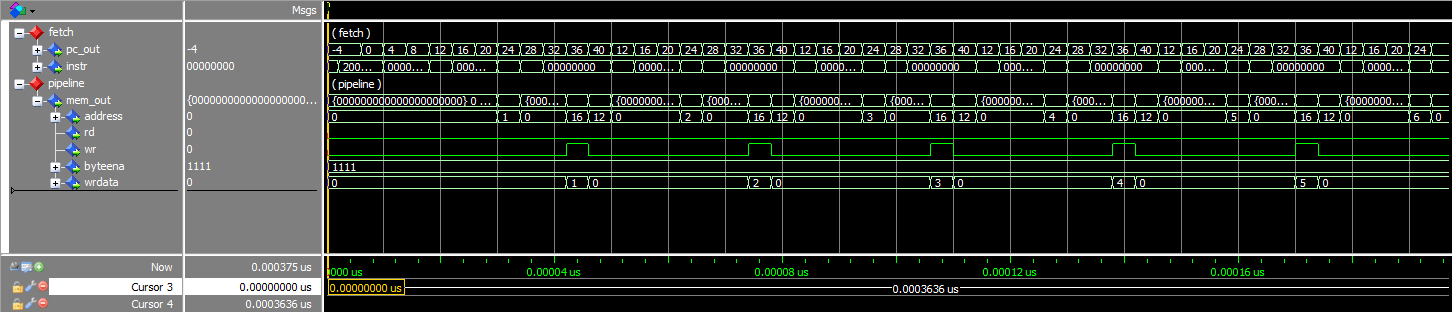
\includegraphics[width=1.0\linewidth]{sim1.png}
  \caption{Simulation screenshot for Listing~\ref{lst:asmnofwd} - five+  loop cycles. Note: Adress and wrdata in deciaml, instr in hex.}
  \label{fig:sim}
\end{figure}

\begin{figure}[ht!]
  \centering
  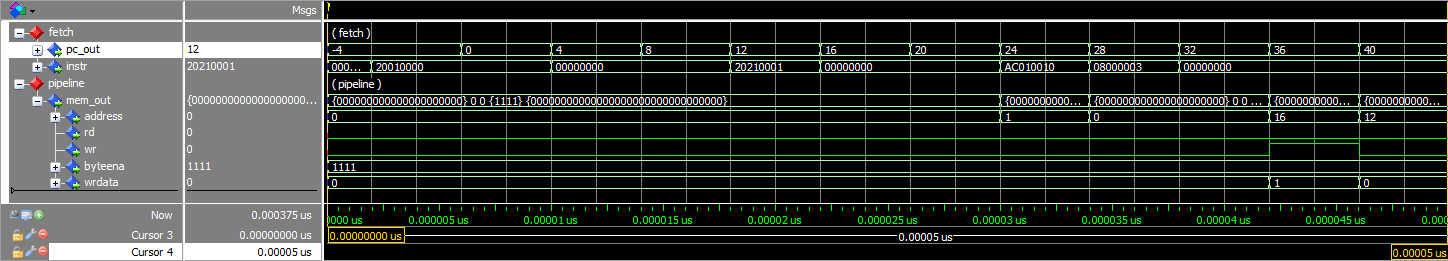
\includegraphics[width=1.0\linewidth]{sim3.png}
  \caption{Simulation screenshot for Listing~\ref{lst:asmnofwd} - first loop cycle.}
  \label{fig:sim}
\end{figure}

Make sure the following signals are visible in Figure~\ref{fig:sim}:
the program counter in the fetch stage, the instruction being fetched,
and the fields \texttt{address}, \texttt{rd}, \texttt{wr},
\texttt{byteena}, and \texttt{wrdata} in the \texttt{mem\_out} signal
coming out of the pipeline.

\begin{lstlisting}[language=,mathescape=false,float=ht,caption={Assembler example without forwarding},label=lst:asmnofwd]
        addi $1, $0, 0
        nop
        nop
loop:
        addi $1, $1, 1
        nop
        nop
        sw $1, 16($0)
        j loop
        nop
        nop
        nop
\end{lstlisting}



